% !TEX root = ../../main.tex
% !TEX encoding = UTF-8 Unicode
\chapter{Event Displays}
\label{ch:eventDisplay}

Atlantis~\cite{Atlantis} event display is a java application which generates a graphical representation of ATLAS events overlaid on the detector geometry. Using energy and position measurements from recorded events, physics objects, trajectories, and energy deposits can be plotted to give an intuitive picture of the event topology and physics processes. 

In the inner detector, charged particle trajectories are shown by colored curved paths: the highest \pt tracks are colored magenta while all others above 1 \pt are shown in light blue. Calorimeter energy deposits in the LAr (Tile) calorimeters are presented as yellow (red) histograms. Electrons (muons) are represented by green (red) solid lines while jets are represented by translucent white cones. The vector sum of the missing transverse energy, \MET, is shown as a light blue arrow.

Three event displays are presented for high $m(WV)$ events which pass the signal region selection of this analysis: highest VBF candidate (\Sect{\ref{sec:high_vbf}}), highest ggF candidate $e-$channel (\Sect{\ref{sec:high_ggf_e}}), and highest ggF candidate $\mu-$channel (\Sect{\ref{sec:high_ggf_m}}). \Tab{\ref{tab:ed_stats_zzzz}} details event information for the three selected events.

\begin{table}[hbtp]
\begin{center}
\begin{tabular}{rrrr}
\hline
 & VBF Candidate & ggF Candidate ($e$) & ggF Candidate ($\mu$) \\ \hline
 \multicolumn{1}{l}{\textbf{Run Information}} & & &\\ 
 Run Number & 308047  &303421 & 302831 \\
 Event Number & 969360152  & 1781248229 & 91880981 \\
 Lumi Block & 244  & 493 & 37 \\
 \multicolumn{1}{l}{\textbf{Kinematic Information}}& & & \\
 $m(WV\rightarrow \ell\nu J)$ [GeV] & 2759.33  & 3854.56 & 3415.38\\
 \MET [GeV]& 362.13  & 1733.75 & 580.00 \\
 \pt(lepton) [GeV]& 777.14 & 70.58 & 939.74 \\
 \pt($W\rightarrow \ell\nu$) [GeV]& 1137.71  & 1763.09 & 1519.64 \\
 $m(J)$\, [GeV] & 88.80  & 108.19 & 114.25 \\
 $D_2^{\beta=1}$ & 1.632 & 2.355 & 1.542\\
 $m^{\text{VBF}}(j,j)$\, [GeV] & 811.55 & --- & --- \\
 $\Delta\eta^{\text{VBF}}(j,j)$ & 5.680 & --- & --- \\ 
 \multicolumn{1}{l}{\textbf{Boson Tagger$^{\dagger}$}} & & & \\
 Pass $D_2^{\beta = 1}$\, 50\,\% (80\,\%) & No (Yes) & No (Yes) &  Yes (Yes)\\
 Pass $W$ mass 50\,\% (80\,\%) & Yes (Yes) & No (No)& No (No) \\
 Pass $Z$ mass 50\,\% (80\,\%) & Yes (Yes)  & No (Yes) & No (Yes)\\
 \hline
\end{tabular}
\caption[Event information for selected high mass events]{Kinematic and selection information for the three high $m(WV)$ events.  For the VBF candidate, $m^{\text{VBF}}$ and $\Delta\eta^{\text{VBF}}$ are the mass and $\eta$ separation of the two selected VBF small-R jets.\\
\,$^{\dagger}$ The SmoothedWZTagger 50\,\% and 80\,\% working points are used to classify the High-Purity and Low-Purity regions. The working points are \pt-dependent and described in \Ch{\ref{ch:event_selection}}.}
\label{tab:ed_stats_zzzz}
\end{center}
\end{table}

\clearpage
\section{Highest VBF Candidate: $2.76\,\TeV$}
\label{sec:high_vbf}
\begin{figure}[h!tbp]
\begin{center}
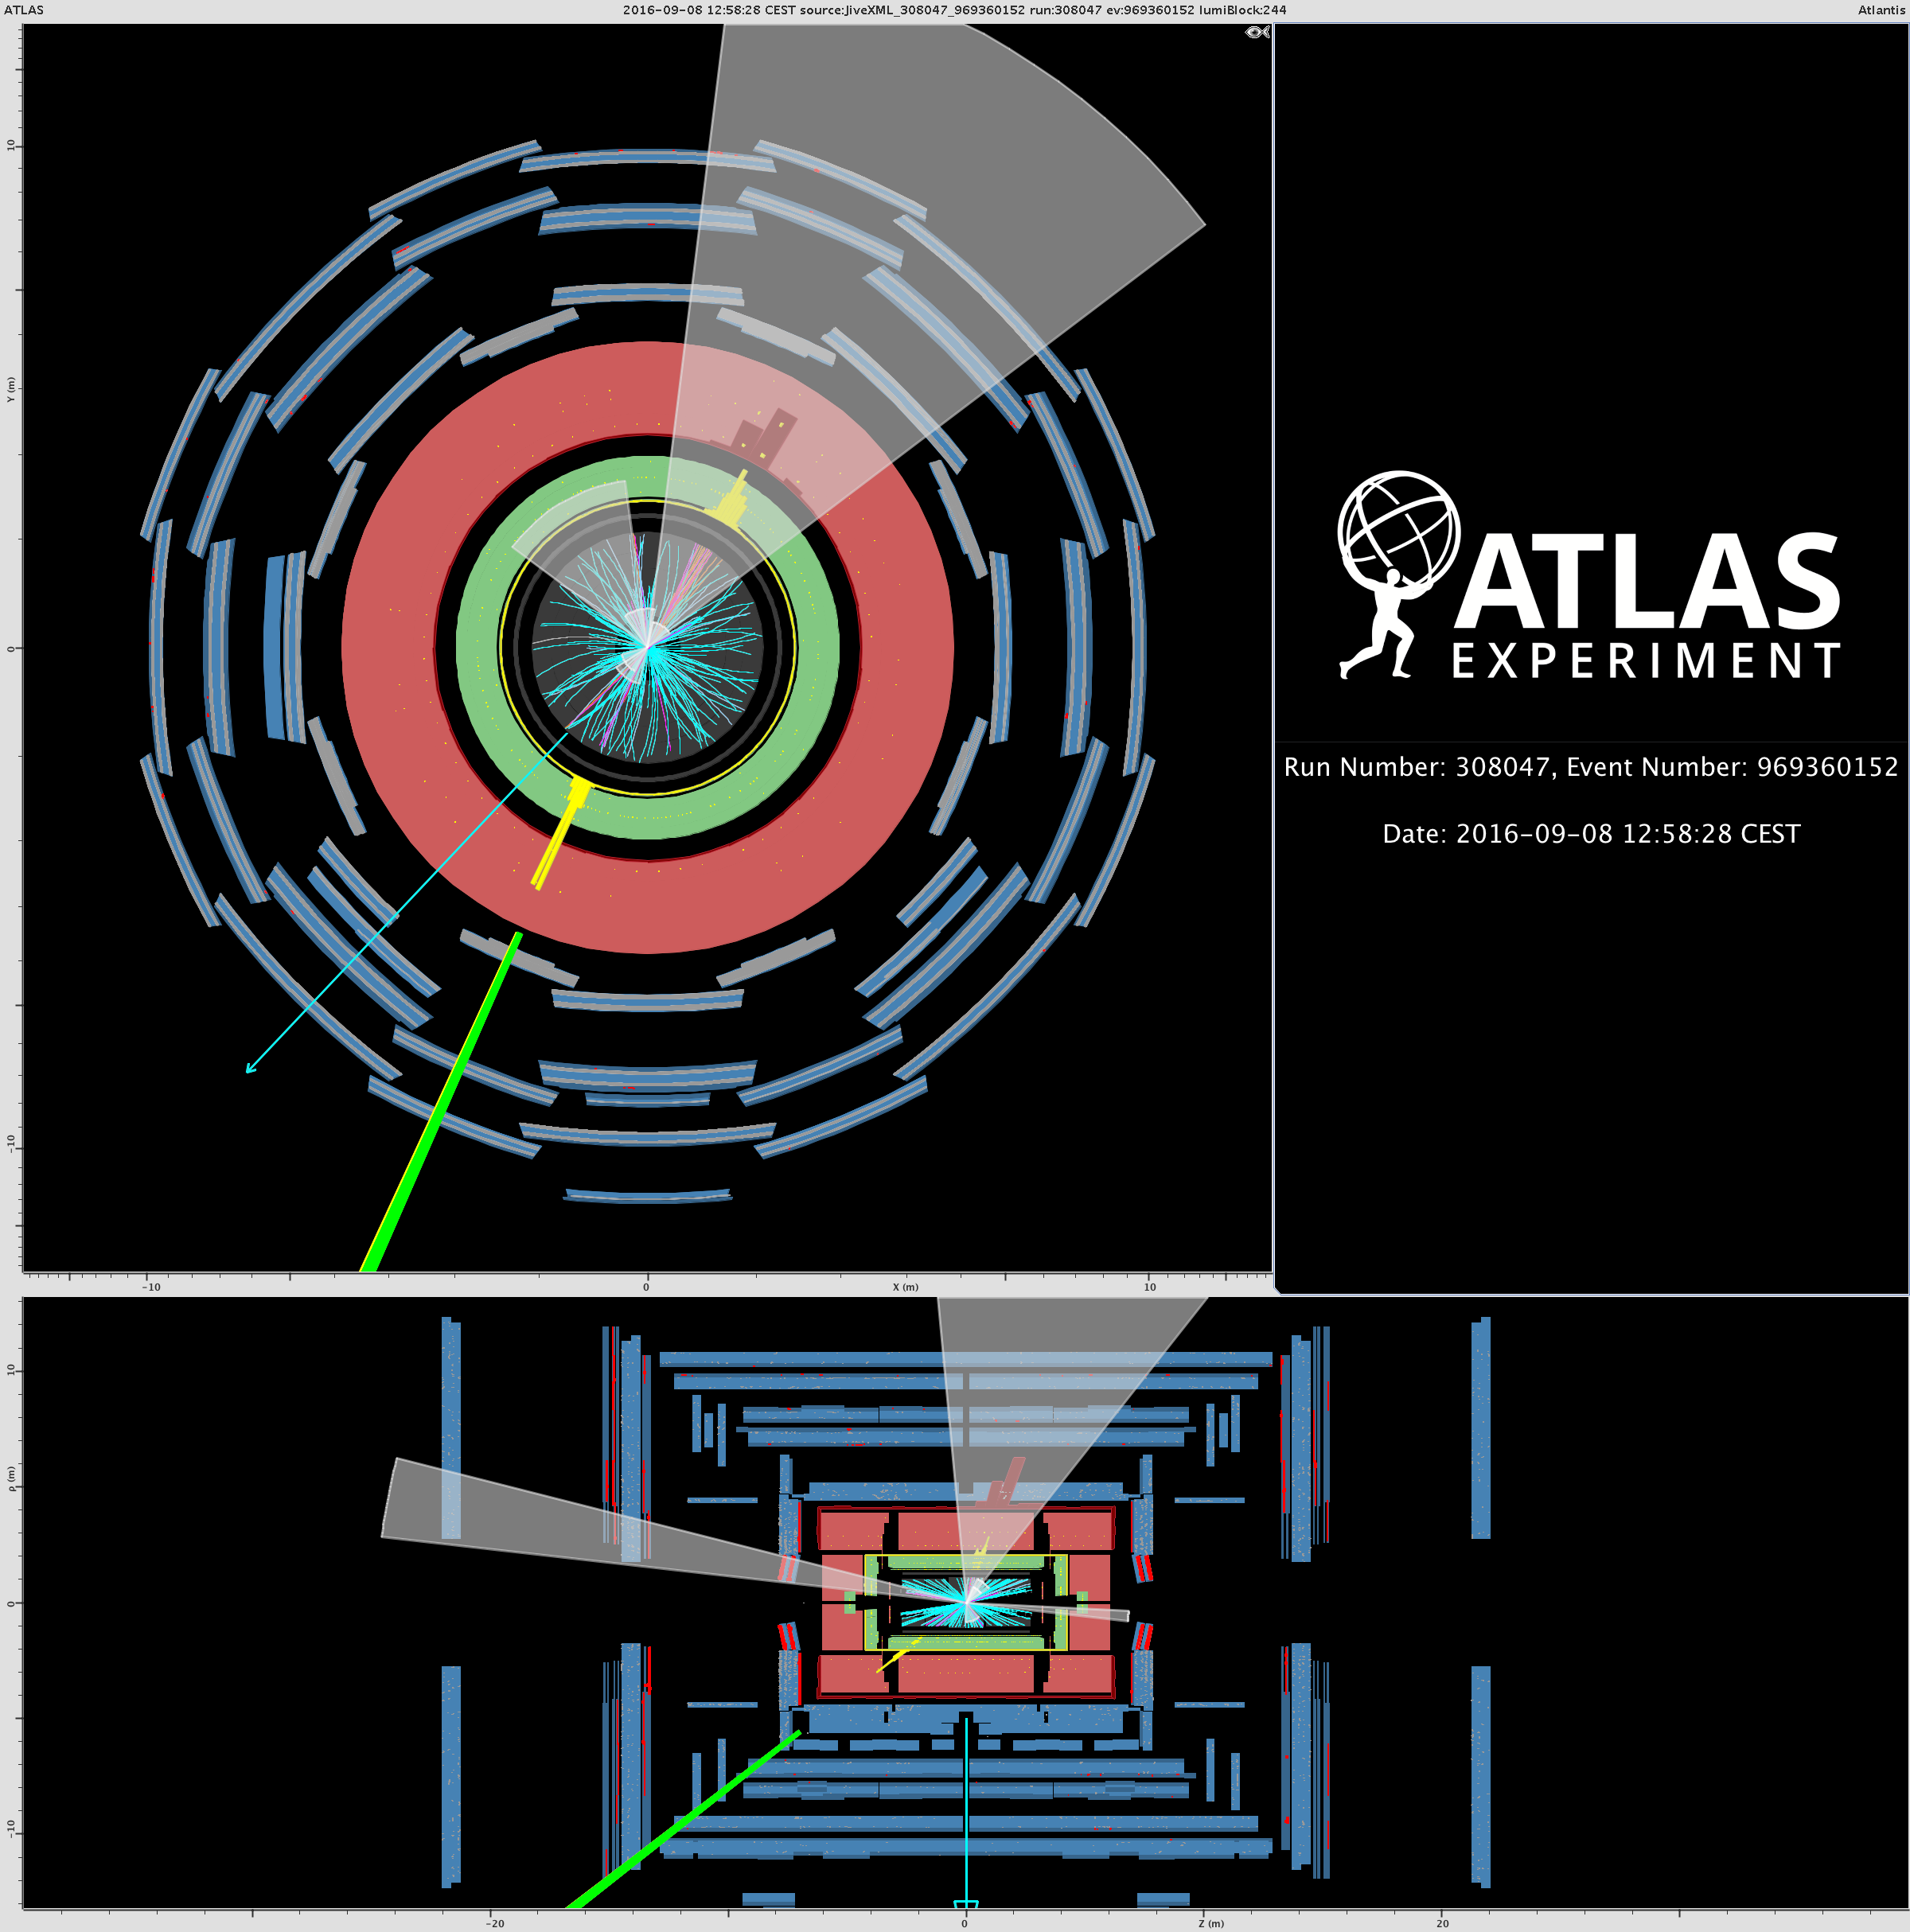
\includegraphics[width=\linewidth]{figures/Appendix/highest_vbf_cand}
\caption[Event display for highest mass candidate (vector boson fusion selection)]{Event display for the event with the largest $m(WV)$ ($2.76\,\TeV$) passing VBF event selection. The top panel shows the event projection in the $R-\phi$ plane looking down the beamline, and the bottom panel shows the event projection in the $R-z$ plane.  In the bottom panel, the two forward VBF jets are clearly visible. The $W\rightarrow \ell\nu$ decay is shown by the electron (green line) and \MET (blue arrow) and is nearly back to back with the hadronically decaying boson which is reconstructed as a central large-R jet (white cone).}
\end{center}
\label{fig:vbf_ed}
\end{figure}

\clearpage
\section{Highest ggF $e$-channel Candidate: $3.85\,\TeV$}
\label{sec:high_ggf_e}

\begin{figure}[h!tbp]
\begin{center}
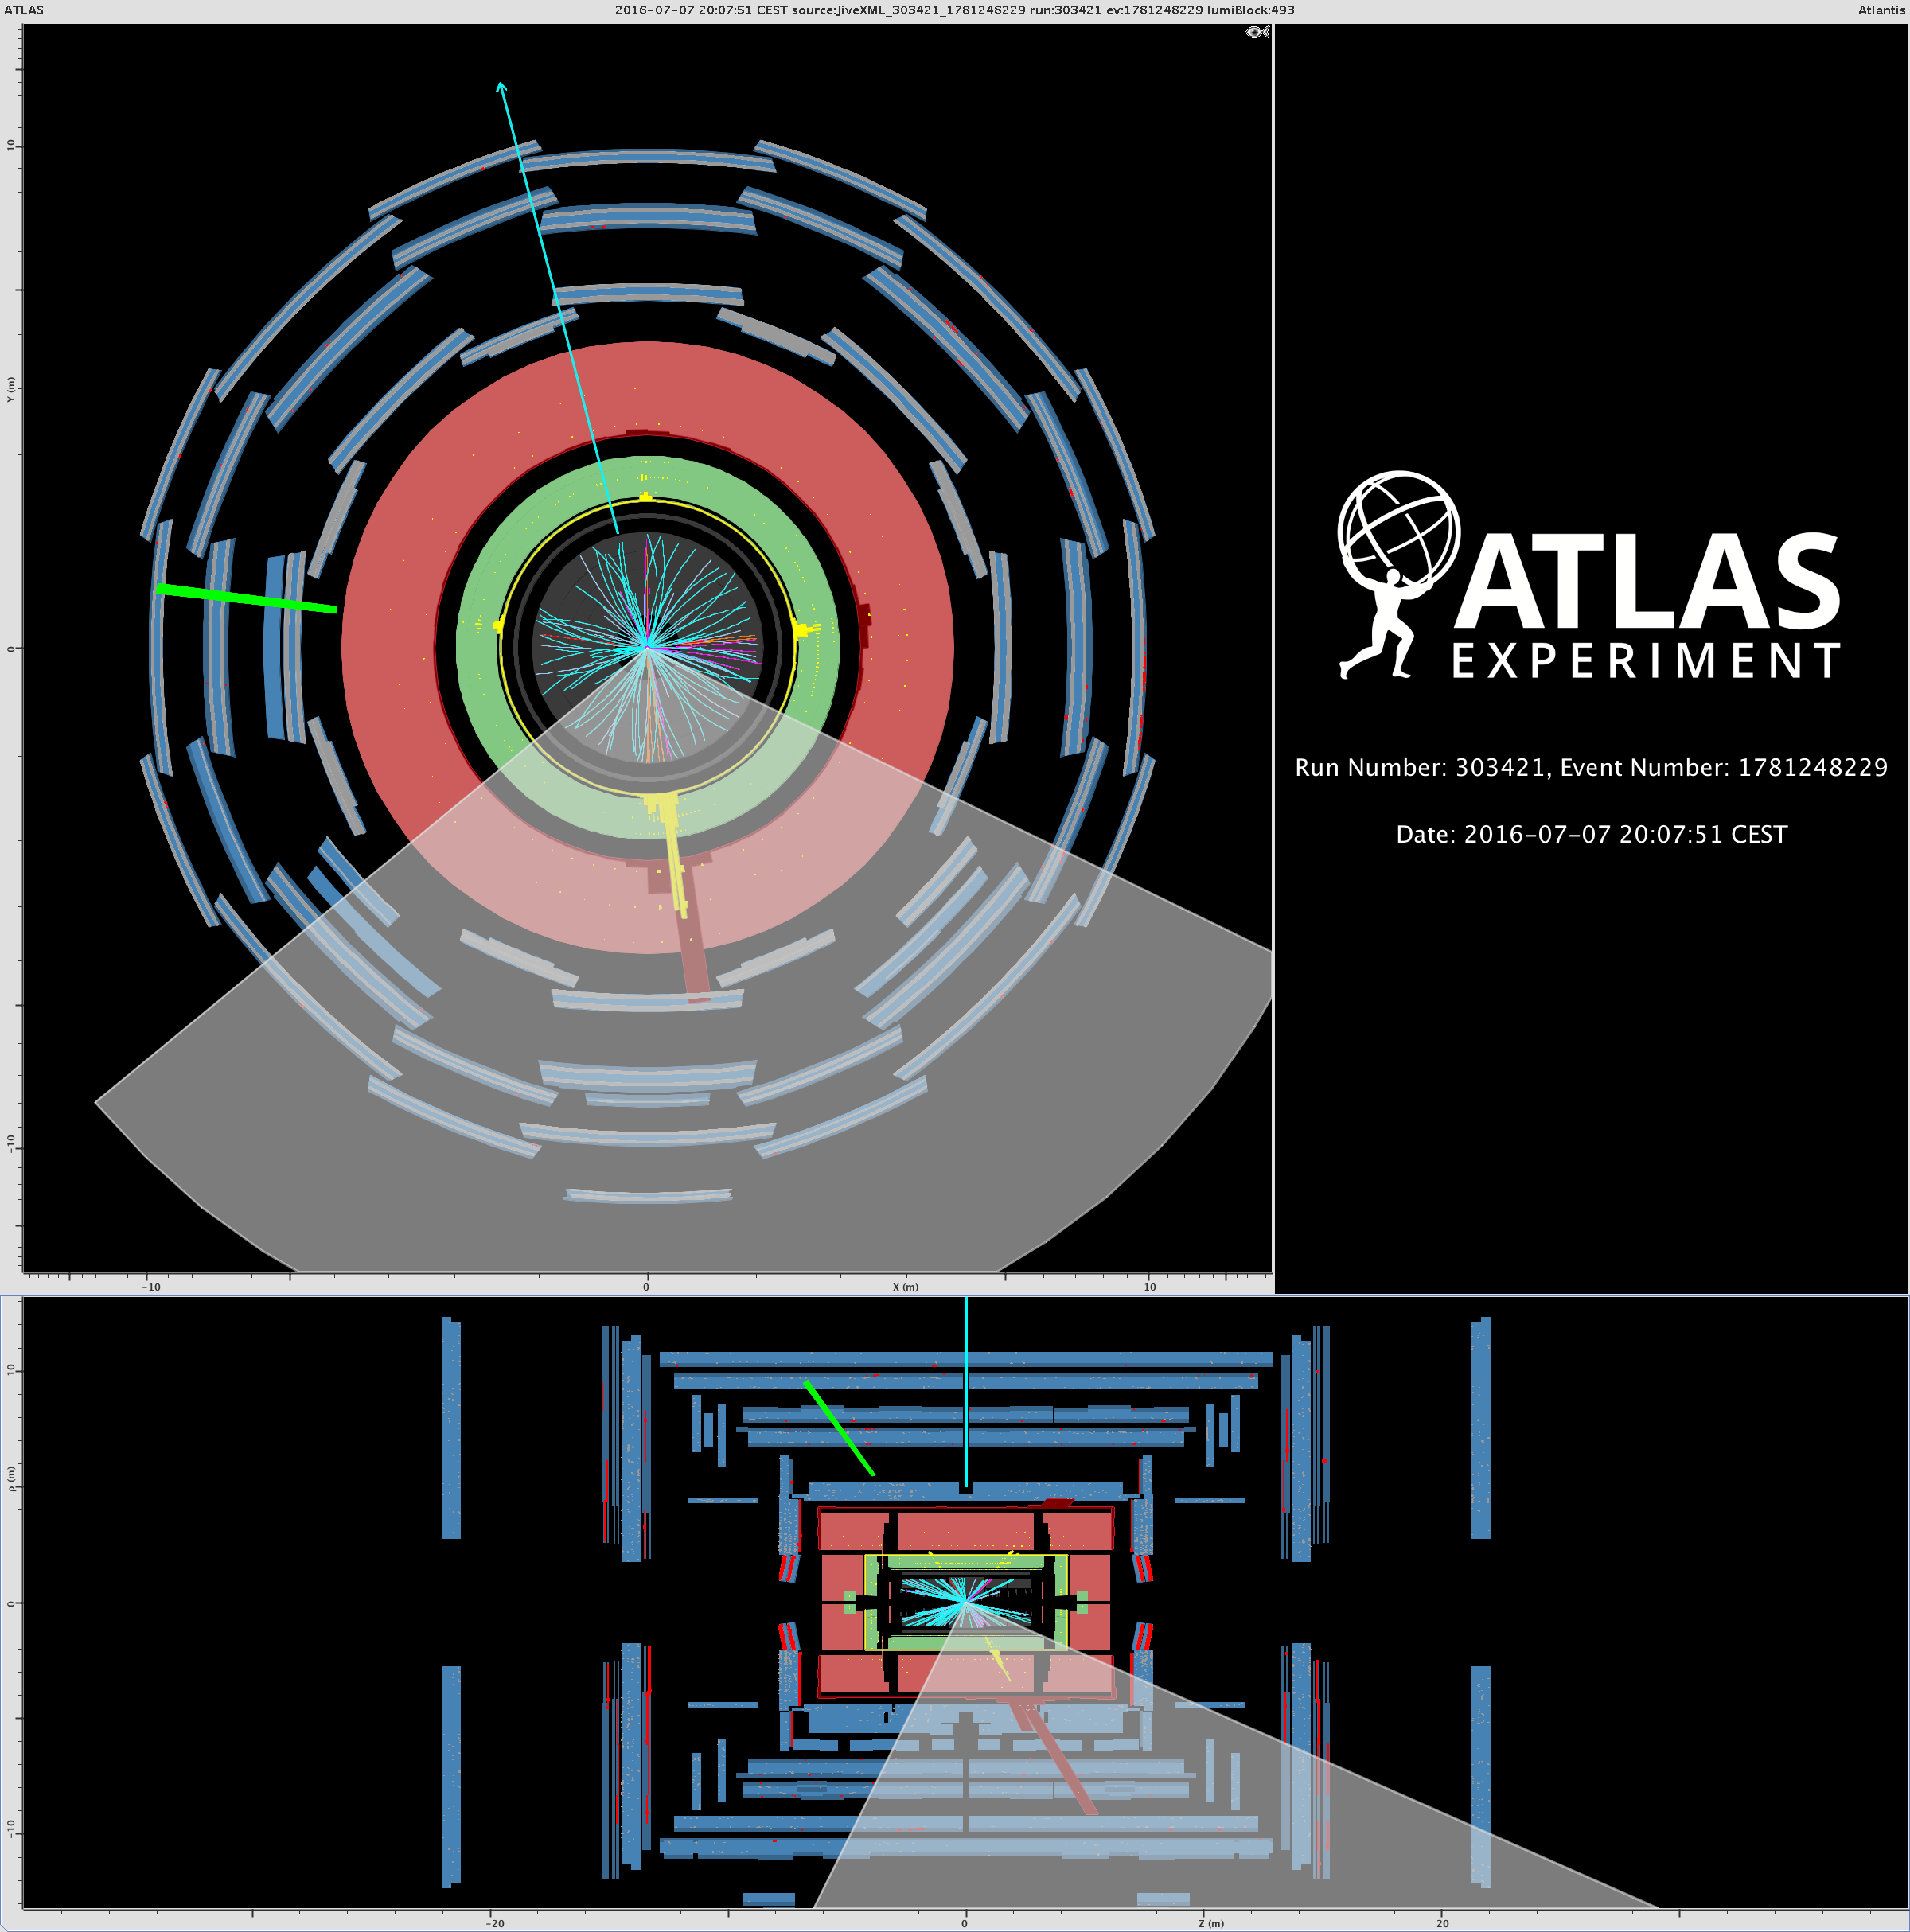
\includegraphics[width=\linewidth]{figures/Appendix/highest_e_candidate}
\caption[Event display for highest mass candidate (gluon-gluon fusion selection, $e$-channel)]{Event display for event with largest $m(WV)$ ($3.85\,\TeV$) passing ggF event selection for the $e$-channel. The top panel shows the event projection in the $R-\phi$ plane looking down the beamline, and the bottom panel shows the event projection in the $R-z$ plane. The $W\rightarrow \ell\nu$ decay is shown by the electron (green line) and \MET (blue arrow) and is nearly back to back with the hadronically decaying boson which is reconstructed as a central large-R jet (white cone).}
\end{center}
\label{fig:ggf_e_ed}
\end{figure}

\clearpage
\section{Highest ggF $\mu$-channel Candidate: $3.41\,\TeV$}
\label{sec:high_ggf_m}

\begin{figure}[h!tbp]
\begin{center}
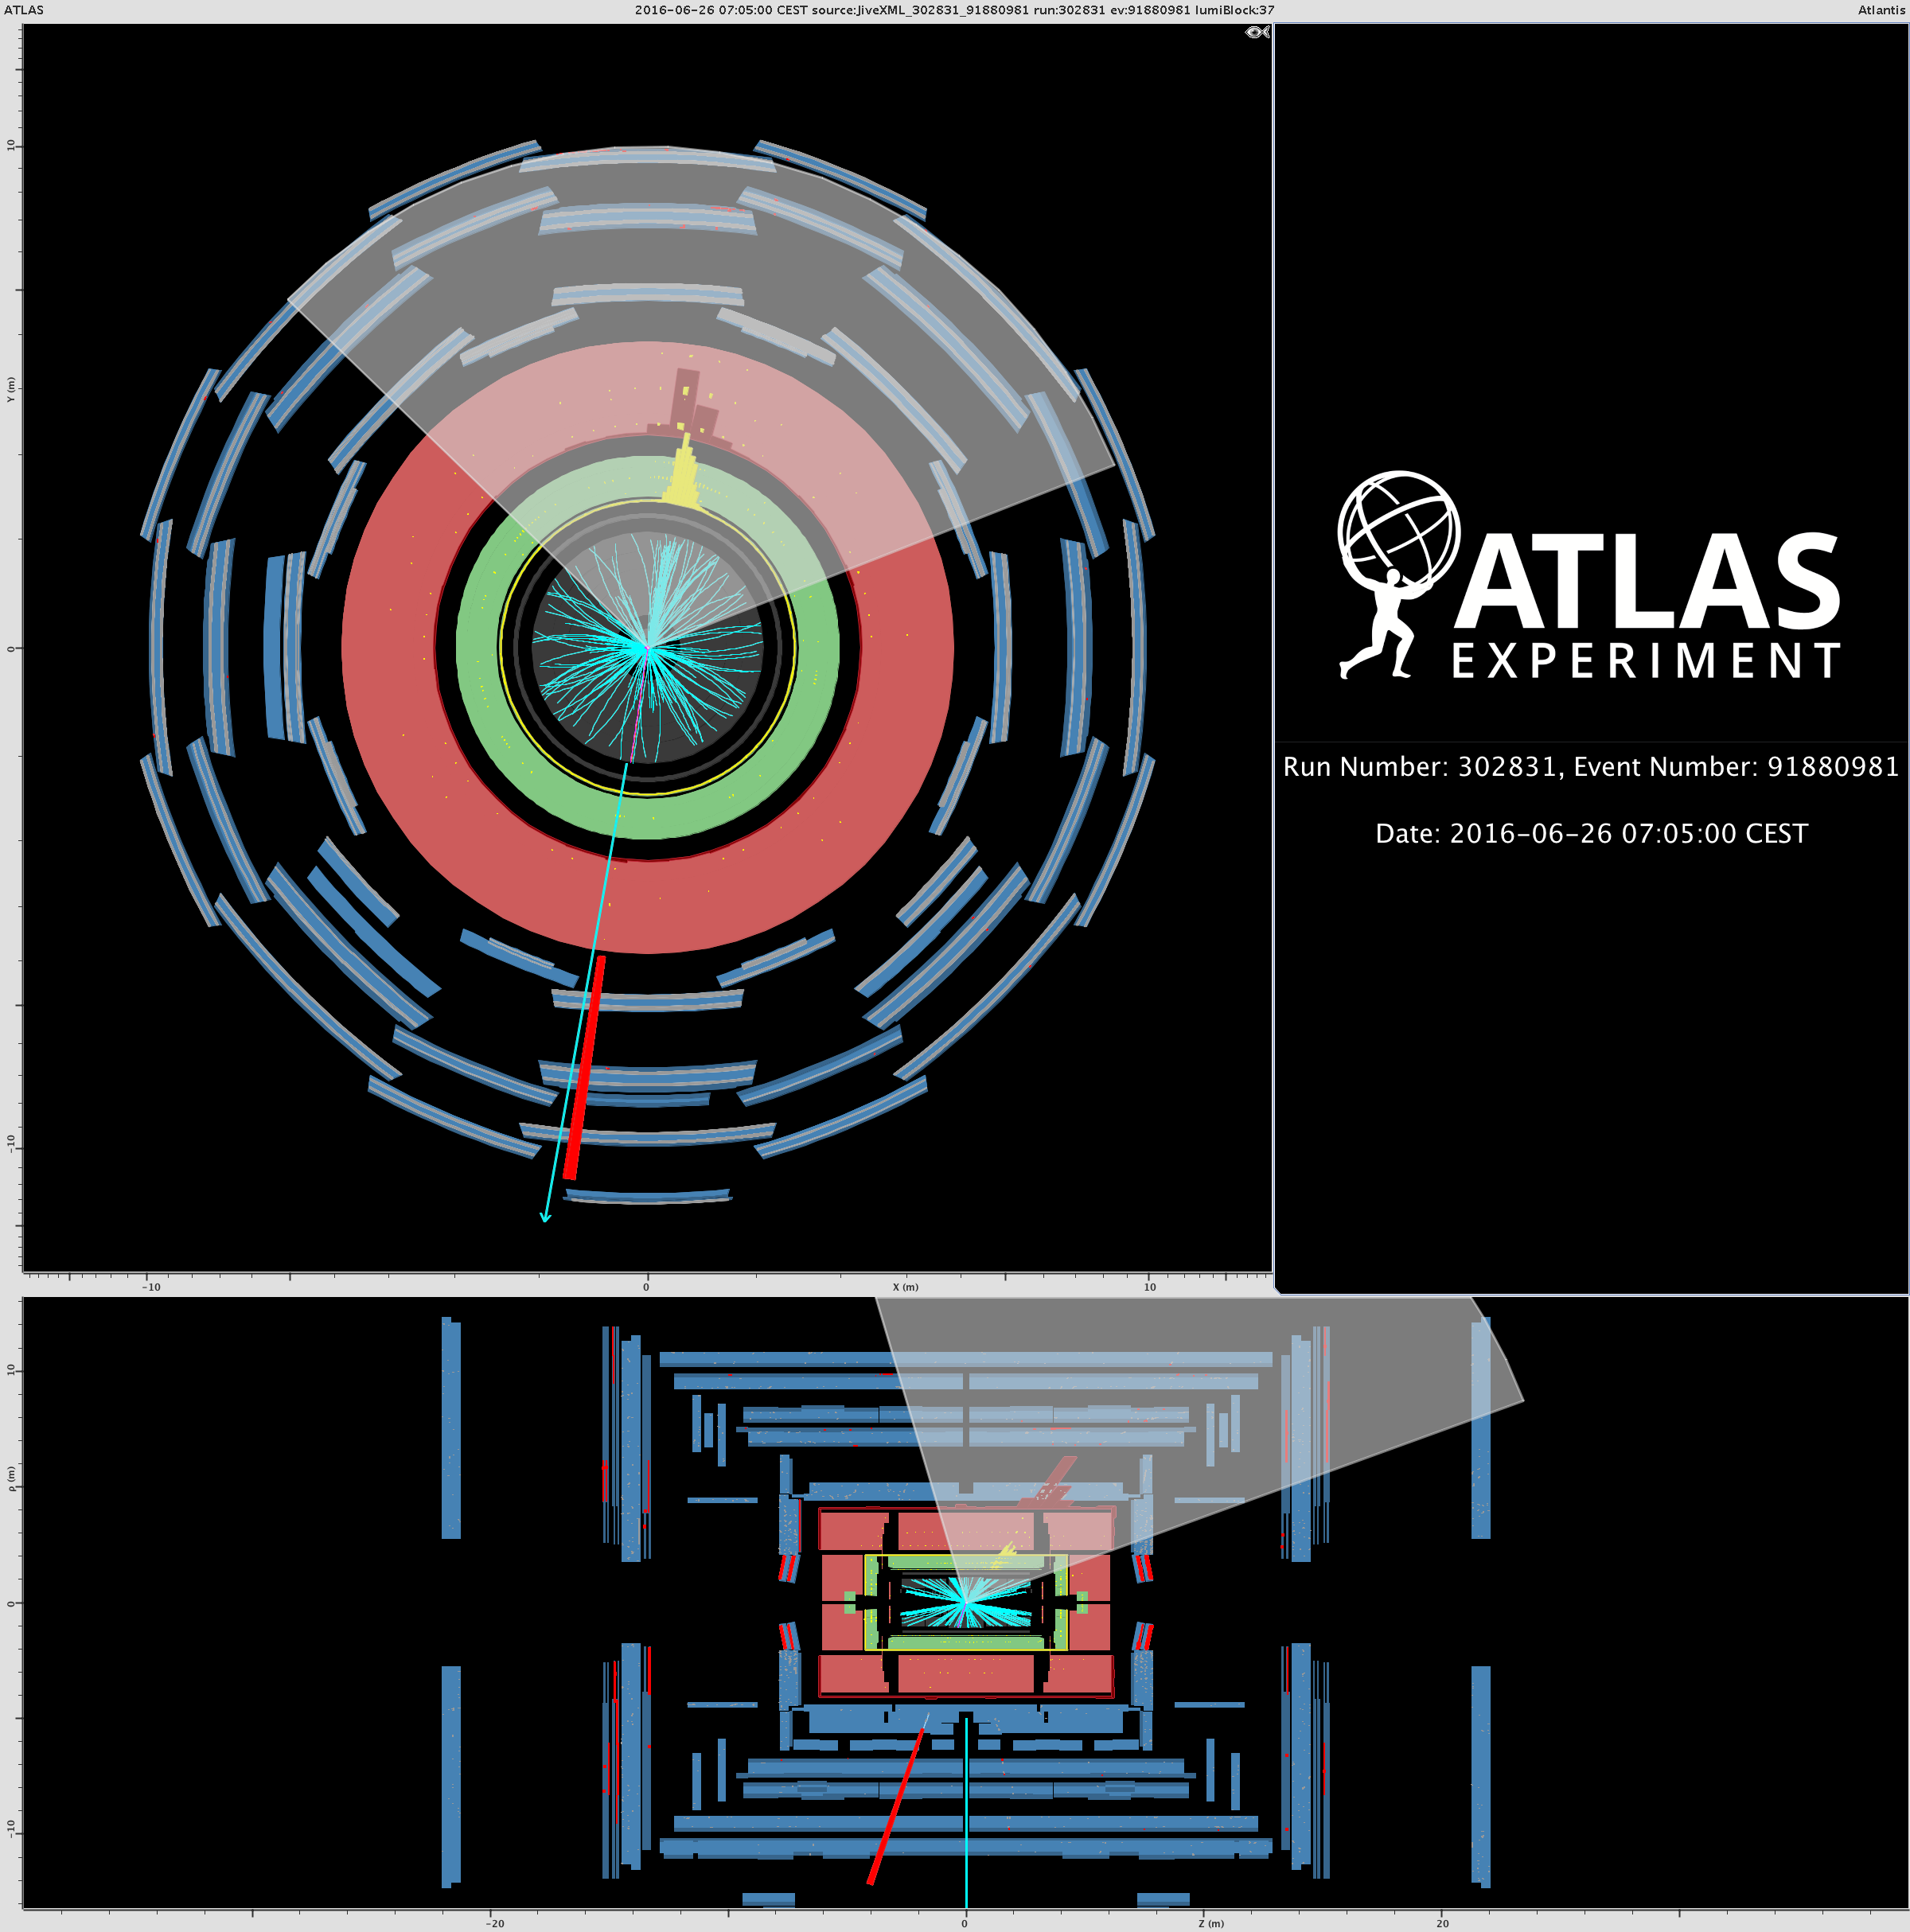
\includegraphics[width=\linewidth]{figures/Appendix/highest_mu_candidate}
\caption[Event display for highest mass candidate (gluon-gluon fusion selection, $\mu$-channel)]{Event display for event with largest $m(WV)$ ($3.41\,\TeV$) passing ggF event selection for the $\mu$-channel. The top panel shows the event projection in the $R-\phi$ plane looking down the beamline, and the bottom panel shows the event projection in the $R-z$ plane. The $W\rightarrow \ell\nu$ decay is shown by the muon (red line) and \MET (blue arrow) and is nearly back to back with the hadronically decaying boson which is reconstructed as a central large-R jet (white cone).}
\end{center}
\label{fig:ggf_mu_ed}
\end{figure}

